\section{ آشنایی با ابزارها و مجموعه داده}
این قسمت به معرفی ابزارهای استفاده شده در این پژوهش می‌پردازد. آشنایی با این ابزارها به درک هرچه بهتر  نحوه‌ی استخراج معیارها  و روند آزمایش کمک می‌کند.

\subsection{مجموعه داده \lr{defect4j}}
 مجموعه‌‌داده‌ی انتخابی به منظور انجام مورد مطالعاتی لازم است که دارای ویژگی‌های زیر باشد:
 \begin{itemize}
 	\item
 	اطلاعات خطاهای پروژه وجود داشته باشد و این اطلاعات نشان دهد که خطا متعلق به کدام پرونده در کدام ثبت است. 
 	\item
 	پروژه‌ها متن-باز باشد تا بتوان با استفاده از \واژه{کد منبع} آنها معیارها را استخراج نمود.
 	\item
 	برای پروژه‌ها موارد آزمون مناسب وجود داشته باشد تا بتوان معیارهای جهش را استخراج کرد.
 \end{itemize}
 در میان مجموعه‌داده‌های موجود مجموعه‌داده‌ی \lr{defects4j} تنها موردی است که تمام ویژگی‌ها را دارد.\\
 
این مجموعه شامل  شش پروژه می‌باشد که این پروژه‌ها  \واژه{متن-باز} هستند و با استفاده از نرم‌افزارهای کنترل نسخه‌ی گیت و svn می‌توان به کدهای آن‌ها در طول فرآیند توسعه‌ی آنها دسترسی پیدا کرد. بجز پروژه‌ی Chart سایرین از سیستم گیت استفاده می‌کنند. همچنین این پروژه به دلیل نداشتن ساختار مناسب کنار گذاشته شد و از پرونده‌های حاوی خطای  موجود در آن استفاده نشد. 
مجموعه‌داده‌ی \چر{defects4j} به صورت یک \واژه{چهارچوب} ارائه شده است که کارهایی بیش از نگهداری اطلاعات درباره‌ی پروژه‌ها انجام می‌دهد. مهم‌ترین  کارهایی که می‌توان به وسیله‌ی این ابزار انجام داد در جدول \ref{tab:defects4j-ops} آمده است. 


\begin{table}[H] 
	\renewcommand*{\arraystretch}{1.3}	
	\centering \caption{عملیات‌های موجود در \چر{defects4j}  }
	\label{tab:defects4j-ops}
	\newcolumntype{C}{>{\centering\arraybackslash} m } 
	\begin{tabular}{ |c|c|}
		
		\hline
		\hline
		نام عملیات  & توضیح
		\\
		\hline
		\hline
		\lr{info } &   نمایش پیکربندی یک پروژه‌ی خاص یا خلاصه‌ی یک خطای خاص
		\\
		\hline
		\lr{checkout} &   وارسی یک نسخه‌ی حاوی خطا یا تعمیر شده از پروژه
		\\
		\hline
		\lr{compile} &   کامپایل کدها و آزمون‌های نوشته شده توسط توسعه‌دهندگان
		\\
		\hline
		\lr{test} &   اجرای یک آزمون یا مجموعه‌ی آزمون در یک نسخه‌ی حاوی خطا یا تعمیر شده از پروژه
		\\
		\hline
		\lr{mutation} &   اجرای تحلیل جهش در یک نسخه‌ی حاوی خطا یا تعمیر شده از پروژه
		\\
		\hline
		
	\end{tabular}
\end{table}

این ابزار در اجرای عملیات‌های بالا دارای محدودیت است و تنها آن‌ها را بر روی ثبت‌های از پیش تعیین شده انجام می‌دهد. ثبت‌های از پیش تعیین شده شامل ثبت‌های حاوی خطا و تعمیر آن خطا می‌باشد. در جدول \ref{tab:defects4j-bugs} اطلاعات مربوط به تعداد خطاهای هر پروژه آمده است. 

\begin{table}[H] 
	\renewcommand*{\arraystretch}{1.3}	
	\centering \caption{پروژه‌های موجود در \چر{defects4j}  }
	\label{tab:defects4j-bugs}
	\newcolumntype{C}{>{\centering\arraybackslash} m } 
	\begin{tabular}{ |c|c|c|}
		
		\hline
		\hline
	نام مختصر &	نام کامل  & تعداد خطا
		\\
		\hline
		\hline
		\lr{Chart } & JFreeChart &	26
		\\
		\hline
		\lr{Closure} & \lr{Closure compiler}	& 133
		\\
		\hline
		\lr{Lang} &   \lr{Apache commons-lang} &	65
		\\
		\hline
		\lr{Math} &  \lr{Apache commons-math} &	106
		\\
		\hline
		\lr{Mockito} &   Mockito &	38
		\\
		\hline
		Time & Joda-Time &	27
		\\
		\hline
	-	& کل  پروژه‌ها &   395
		\\
		\hline
		
	\end{tabular}
\end{table}


به منظور نصب و راه اندازی ابزار  \lr{defects4j} ابتدا از صفحه‌ی \نام{گیت‌هاب}{Github} آن  کدهای مربوطه دریافت می‌شود. سپس باید  دستوراتی را اجرا کرد تا سایر متعلقات دریافت شود. این تعلقات شامل مخزن نرم‌افزاری مربوط به شش پروژه‌ی یاد شده است که کدهای پروژه‌ها در آن قرار دارد. نکته‌ی قابل توجه در این ابزار این است  که بجز  دستور info سایر دستورات عملیات‌های مربوط را بر روی کامپیوتر کاربر انجام می‌دهد و خروجی را نمایش  داده می‌شود، نه اینکه از یک پایگاه داده اطلاعات را صرفاً بارخوانی کند. \\
در نیازمندی‌های این ابزار اشاره شده که باید از جاوا نسخه‌ی ۷ استفاده شود. اما مسأله‌ای که به آن اشاره نشده توزیع‌کننده‌ی جاوا است. جاوا دو توزیع کننده ی عمده دارد. یکی OpenJDK و دیگری Oracle می‌باشد. با استفاده از OpenJDK ابزار \lr{defects4j} و ابزارهایی که به آن وابسته است به خوبی کار نمی‌کنند. به عنوان مثال برخی مجموعه آزمون‌ها که باید بدون خطا اجرا شوند به دلیل نبود  \واژه[وابستگی‌های]{وابستگی} لازم با شکست مواجه می شوند. \\ 
راه ارتباط با این ابزار \واژه{خط دستور}‌ می‌باشد و  یک نمونه‌  از دستورات قابل استفاده در این ابزار  در شکل  \ref{fig:d4j-info-command} است که این دستور اطلاعات مربوط به پروژه‌ی Lang و خطای شماره‌ی یک را خواهد داد. 
\begin{latin}
	\flushleft
defects4j info -p Lang -b 1
\end{latin}

\begin{figure}[H]
	\centering
	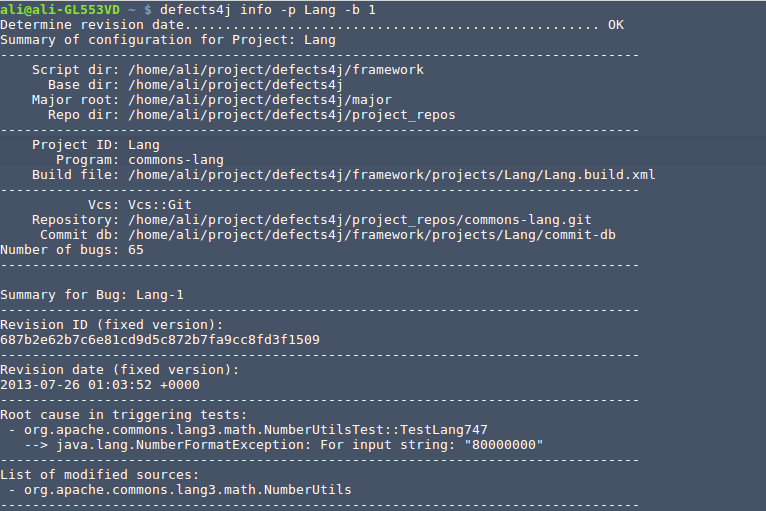
\includegraphics[width=.8\textwidth]{img/case_study/d4j-info-commadn.png}
	\caption{اجرای دستور info در \lr{defects4j}}
	\label{fig:d4j-info-command}
\end{figure}

\subsection{ابزار Major}
\label{sec:tools-major}

این ابزار جهت تولید جهش‌یافته و تحلیل جهش استفاده می‌شود. یک ابزار دیگر در این حوزه 
\نام{پیت}{PIT - \url{http://pitest.org/}} می‌باشد اما به دلیل سازگاری ابزار \lr{defects4j} با Major و نیز قابلیت‌های ویژه‌ی آن از این ابزار استفاده شد.
چند مورد از ویژگی‌های مهم ابزار Major عبارتند از :
\begin{itemize}

\item
 راحتی استفاده  به دلیل نیاز به دستورات کمتر نسبت به پیت
\item
امکان اجرای تحلیل جهش در پروژه‌هایی که از \نام{گریدل}{Gradle} استفاده می‌کنند
\item
 مجموعه عملگرهای کاملتر
\item
انعطاف در پیکربندی : امکان انجام تحلیل تنها برای یک کلاس یا تابع، تنظیمات ساده و کامل جهت مشخص کردن مجموعه عملگرها
\end{itemize}
لازم به ذکر است که این ابزار از کامپایلر‌ مخصوص به خود جهت کامپایل برنامه و ساخت جهش‌یافته استفاده می‌کند که گسترش یافته‌ی یک کامپایلر جاوا است. 
استفاده از این ابزار را می‌توان در سه مرحله خلاصه کرد :
\begin{enumerate}
\item

\textbf{پیکربندی تولید جهش‌یافته به وسیله‌ی دستورات \lr{MML}: }
این ابزار برای مشخص نمودن اینکه از چه عملگرهایی استفاده شود و آن‌ها در چه محل‌هایی از برنامه به کار گرفته شوند یک زبان ساده ابداع کرده است به نام MML که یک کامپایلر نیز دارد. ابتدا کد MML نوشته می‌شود و سپس با MMLC کامپایل می‌شود و نتیجه به عنوان یکی از پارامترها  در هنگام فراخوانی به ابزار  Major ارسال می شود. \\

نمونه‌ای از این کد در شکل \ref{fig:major-mml} آمده است. در بلاک targetOp مجموعه‌ی عملگرها مشخص می‌شود و در خط آخر محلی که عملگرهای جهش مشخص شده عمل می‌کند. در واقع تنها برای محل مشخص شده جهش‌یافته تولید می‌شود. در بلاک targetOP ابتدا مشخص می‌شود که عملگرهای باینری موجود در برنامه به چه عملگرهای دیگری تبدیل شود. همچنین امکان مشخص کردن نحوه‌ی تبدیل عملگرهای یگانی با دستو UNI به جای BIN وجود دارد. سپس عباراتی که امکان حذف آنها وجود دارد مشخص می‌شود که در شکل امکان حدف خروجی توابع مشخص شده است. در قسمت آخر مجموعه عملگرهای جهش قابل استفاده مشخص شده که در شکل عملگرهای حذف عبارت، جایگزنی عملگر شرطی و جایگزینی عملگر رابطه‌ای به کار گرفته شده است. مجموعه‌ی عملگرهای موجود در این ابزار در \cite{just2014major} آمده است. 

\begin{figure}[H]
	\centering
	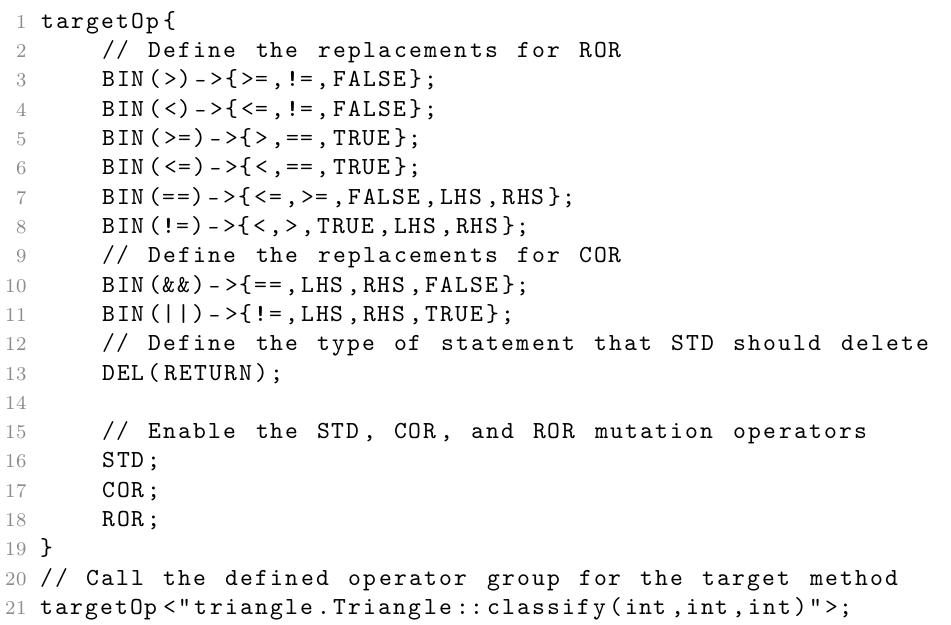
\includegraphics[width=.8\textwidth]{img/case_study/major-mml.png}
	\caption{نمونه کد MML در Major}
	\label{fig:major-mml}
\end{figure}
\item 	
\textbf{تولید جهش‌یافته‌ها:}
 همانطور که اشاره شد ابزار Major جهت تولید نسخ جهش‌یافته نیاز به کامپایل پروژه دارد. امروزه پروژه‌های نرم‌افزاری از جمله پروژه‌های موجود در \lr{defects4j} از ابزارهایی استفاده می‌کنند که فرآیند ساخت را خودکارسازی می‌کنند. فرآیند ساخت به طور کلی شامل مراحل زیر است:
\begin{itemize}
	\item پاک سازی  پوشه‌های کاری، از پرونده‌های ساخت‌های قبلی
	\item 
	معرفی‌ وابستگی‌ها و کامپال پروژه
	\item
	معرفی وابستگی‌ها و کامپایل موارد آزمون
	\item
	اجرای موارد آزمون و ارائه‌ی گزارش
\end{itemize}
سه نوع از مهم ترین ابزارهای خودکارسازی مورد استفاده در صنعت عبارتند از Ant ،  Maven و \lr{Gradle}. در پروژه‌های مورد مطالعه نیز این سه نوع به کار گرفته شده است.  
هر یک از روش‌ها خودکارسازی دارای دستورات مربوط به خود می‌باشد  و برای تولید جهش‌یافته باید متناسب با آنها عمل نمود که در زیر خلاصه شده است. 
\begin{itemize}
	\item
	Ant : 
	این دسته از پروژه‌ها دارای یک پرونده به نام build.xml است که دستورات لازم جهت پیکربندی و انجام عملیات ساخت در آن قرار دارد. به منظور تولید جهش‌یافته کافیست کامپایلر مورد استفاده در قسمت کامپایل پروژه را کامپایلر توسعه‌یافته‌ی Major قرار داد و پارامترهای لازم به آن ارسال شود. 
	\item Maven : 
	در این دسته از پروژه‌ها دستورات لازم در پرونده‌ی pom.xml قرار دارد.  به وسیله‌ی  یک \واژه{افزونه} در ابزار Maven این پرونده تبدیل به یک پرونده build.xml می‌شود که قابل استفاده توسط ابزار Ant است. پس از این تبدیل مشابه حالت قبل عمل می‌شود. 	
	\item Gragle : 
	در این دسته از پروژه‌ها دستورات لازم در پرونده‌ی  build.gradle قرار دارد.  به منظور تولید جهش‌یافته کافیست کامپایلر مورد استفاده در قسمت کامپایل پروژه را کامپایلر توسعه‌یافته‌ی Major قرار داد و پارامترهای لازم به آن ارسال شود. 
\end{itemize}

نمونه‌ای از حاصل اجرای  عملیات جهش برای یک پرونده در شکل \ref{fig:major-mutant}  آمده است   که نشان می‌دهد ۸۶ جهش یافته تولید شده است. همچینین ابزار یک پرونده به نام mutants.log تولید می‌کند که نشان می‌دهد چه جهش‌یافته‌هایی در کجا تولید شده‌اند. نمونه‌ای از محتویات این پرونده در شکل \ref{fig:major-log}  آمده است. 

\begin{figure}[H]
	\centering
	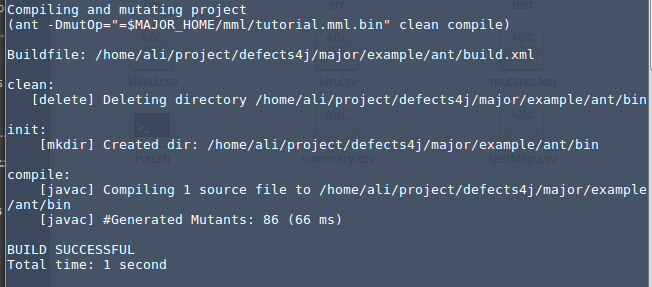
\includegraphics[width=.8\textwidth]{img/case_study/major-mutant.png}
	\caption{اجرای عملیات جهش برای یک پرونده}
	\label{fig:major-mutant}
\end{figure}

\begin{figure}[H]
	\centering
	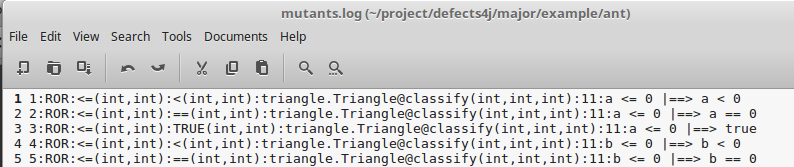
\includegraphics[width=\textwidth]{img/case_study/major-log.png}
	\caption{نمونه‌ای از پرونده‌ی mutants.log}
	\label{fig:major-log}
\end{figure}

\item
\textbf{ اجرای تحلیل جهش:}
 ابتدا پرونده‌های آزمون کامپایل می‌شود و سپس هر مجموعه آزمون بر روی جهش‌یافته‌هایی که تاکنون کشته نشده‌اند اجرا می‌شود. در پایان نتایج  در خروجی چاپ می‌شوند. همچنین نتایج  در پرونده‌های با پسوند csv قرار می‌گیرد. نمونه‌ای از اجرای تحلیل جهش در شکل \ref{fig:major-analysis} و پرونده‌ی نتایج خروجی در شکل \ref{fig:major-results} نشان داده شده.
 
 \begin{figure}[H]
 	\centering
 	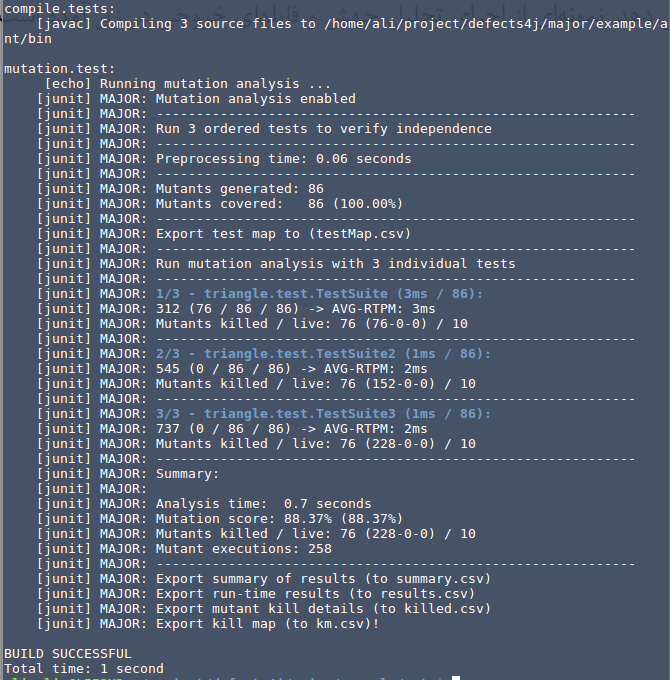
\includegraphics[width=.8\textwidth]{img/case_study/major-analysis.png}
 	\caption{اجرای تحلیل جهش}
 	\label{fig:major-analysis}
 \end{figure}
 
 \begin{figure}[H]
 	\centering
 	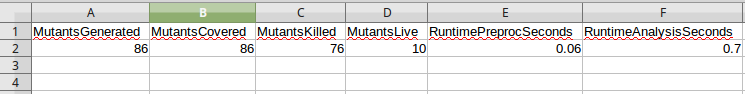
\includegraphics[width=.8\textwidth]{img/case_study/major-results.png}
 	\caption{نتایج خروجی تحلیل جهش}
 	\label{fig:major-results}
 \end{figure}

\end{enumerate}


\subsection{کتابخانه‌ی Jgit}
این کتابخانه جهت کار با مخازن نرم‌افزاری  که از نوع گیت هستند به کار گرفته می‌شود و به زبان جاوا است. تمام عملیات‌های مهم و اساسی که در نرم‌افزار اصلی گیت وجود دارد در این کتابخانه نیز قابل انجام است. مشکلی که کار با این کتابخانه دارد نبود منابع آموزشی به اندازه‌ی کافی است. چراکه کاربران زیادی ندارد و آموزش‌های ابتدایی معمولاً نیازهای عموم کاربران را بر طرف می‌کند. 
\subsection{چارچوب Hibernate }
به وسیله‌ی این چارچوب می‌توان  اشیاء موجود در برنامه‌ی جاوا را به داده‌های موجود در پایگاه داده تبدیل کرد. اصطلاحاً به این ابزار ها \نام{ORM}{Object Relational Mapping} می‌گویند. مزیت استفاده از این نوع از ابزارها این است که ارتباط با پایگاه داده ساده‌تر خواهد شد و حجم کدهای لازم کاهش چشم‌گیری خوهد داشت. همچنین این ابزارها اشیاء را در حافظه‌ی موقت مدیریت می‌کنند و حجم کاری پایگاه داده کاسته می‌شود. 